\documentclass[12pt]{beamer}

\hypersetup{colorlinks=true,linkcolor=red}
\usetheme{default}
\usecolortheme{albatross}

\usepackage[utf8]{inputenc}
\usepackage[russian,english]{babel}
\usepackage[T2A]{fontenc}
\usepackage{hyperref}
\usepackage[final]{listings}
\usepackage{breakurl}
\usepackage{cite}
\usepackage{perpage}

\graphicspath{{img/}}

\def\Url\Breaks{\do\/\do-}
\lstset{
  frame=single,
  breaklines=true,
  basicstyle=\tiny,
  postbreak=\raisebox{0ex}{\ensuremath{\hookrightarrow\space}},
  numbers=left
}

\MakePerPage{footnote}

\title{Operating Systems}
\subtitle{Threads, Processes and Scheduling}
\author{Me}
\date{\today}

\begin{document}
  \begin{frame}
    \titlepage
  \end{frame}

  \begin{frame}
\frametitle{Поток исполнения}
\begin{itemize}
  \item Поток исполнения (aka поток) - память содержащая команды и некоторый
  контекст, определяющий состояние потока исполнения
  \begin{itemize}
    \item набор команд и то что нужно для их исполнения.
  \end{itemize}
  \item Контекст потока - окружение в котором исполняются команды и состояние
  CPU:
  \begin{itemize}
    \item доступная память:
    \begin{itemize}
      \item таблица страниц определяет всю доступную память (если вы ее
      используете);
      \item память с командами и данными;
      \item стек;
    \end{itemize}
    \item регистры процессора.
  \end{itemize}
\end{itemize}
\end{frame}

\begin{frame}
\frametitle{Память потока}
\begin{itemize}
  \item Различные потоки исполнения \emph{могут} "разделять" общую память:
  \begin{itemize}
    \item использовать один и тот же набор команд;
    \item работать с одними и теми же данными;
    \item однако потоки могут быть и изолированы друг от друга, например, иметь
    свою таблицу страниц.
  \end{itemize}
  \item Стек у каждого потока свой:
  \begin{itemize}
    \item стек важная область памяти для исполнения команд потока;
    \item стек хранит локальные переменные функций;
    \item на стек, \emph{обычно}, сохраняются адреса возврата при вызове
    функций.
  \end{itemize}
\end{itemize}
\end{frame}

\begin{frame}
\frametitle{Состояние CPU}
\begin{itemize}
  \item Состояние CPU включает:
  \begin{itemize}
    \item регистры общего назначения:
    \begin{itemize}
      \item например, для x86-64 это регистры RAX, RBX, RCX, RDX, RDI, RSI,
      RBP, RSP, R9-R15;
    \end{itemize}
    \item флаговый регистр (или регистры):
    \begin{itemize}
      \item регистры флагов используются для организации условных переходов или
      условного исполнения;
      \item например, для x86-64 это регистр RFLAGS;
    \end{itemize}
    \item прочие регистры, участвующие в вычислениях:
    \begin{itemize}
      \item например, xmm/avx/прочие регистры x86 используемые для
      floating-point арифметики и SIMD инструкций, которые не будут
      интересовать нас в домашних заданиях.
    \end{itemize}
  \end{itemize}
\end{itemize}
\end{frame}

\begin{frame}
\frametitle{Многопоточность}
\begin{itemize}
  \item Одновременно могут исполняться сразу несколько потоков:
  \begin{itemize}
    \item если на одном кристалле находится сразу несколько полноценных или не
    очень (aka Hyper Threading) вычислительных ядер;
    \item если у вас просто несколько CPU в системе.
  \end{itemize}
  \item Потоки могут исполняться \emph{почти} одновременно:
  \begin{itemize}
    \item одновременность в контексте многопточности - плохое слово (вообще
    понятие времени очень странное в данном контексте);
    \item в каждый момент времени на конкретном CPU исполняется только один
    поток, но между потоками можно быстро переключаться создавая иллюзию
    одновременной работы.
  \end{itemize}
\end{itemize}
\end{frame}

\begin{frame}
\frametitle{Кооперативная и вытесняющая многопточность}
\begin{itemize}
  \item Кооперативная многопоточность
  \begin{itemize}
    \item поток работает на CPU до тех пор, пока он сам не решит "отдать" CPU
    кому-нибудь другому;
    \item часто в некоторых контекстах такие потоки называют корутинами;
    \item считается, что программировать используя кооперативную многопточность
    проще (впрочем, это очень-очень-очень спорное утверждение).
  \end{itemize}
  \item Вытесняющая многопоточность
  \begin{itemize}
    \item поток может быть смещен (вытеснен) c CPU в любой момент без
    предупреждения;
    \item например, ОС может смещать поток с CPU, если он отработал достаточно
    долго;
    \item поток все еще может сам отдать CPU.
  \end{itemize}
\end{itemize}
\end{frame}

\begin{frame}
\frametitle{Переключенние потоков}
\begin{itemize}
  \item Для переключения потоков, очевидно, нужно подменить контекст одного
  потока, контекстом другого потока и передать управление коду другого потока
  \begin{itemize}
    \item чтобы уметь переключиться назад на старый поток необходимо сохранить
    его контекст, чтобы его можно было восстановить;
    \item переключением с одного потока на другой поток занимается какой-то
    код, этот код тоже использует регистры и какую-то память;
    \item соответственно, это код не должен в процессе сохранения состояния
    испортить само состояние;
    \item соответственно, код переключающий потоки должен быть доступен в каждом
    потоке - все потоки должны иметь какую-то общую память.
  \end{itemize}
\end{itemize}
\end{frame}

\begin{frame}[fragile]
\frametitle{Пример переключения для x86}
\begin{columns}
  \begin{column}{0.4\linewidth}
    \begin{lstlisting}
    .text
switch_threads:
    pushq %rbx
    pushq %rbp
    pushq %r12
    pushq %r13
    pushq %r14
    pushq %r15
    pushfq

    movq %rsp, (%rdi)
    movq %rsi, %rsp

    popfq
    popq %r15
    popq %r14
    popq %r13
    popq %r12
    popq %rbp
    popq %rbx

    ret
    \end{lstlisting}
  \end{column}
  \begin{column}{0.6\linewidth}
    \begin{lstlisting}
void switch_thread(void **prev,void *next);
    \end{lstlisting}
    \begin{itemize}
      \item сохраняет состояние старого потока на стек:
      \begin{itemize}
        \item через \emph{prev} (регистр rdi) возвращается указатель на
        сохраненное состояние;
        \item \emph{next} (регистр rsi) - указатель на сохраненное состояние
        нового потока;
      \end{itemize}
    \end{itemize}
  \end{column}
\end{columns}
\end{frame}

\begin{frame}
\frametitle{Пример переключения для x86}
\begin{center}
  
\includegraphics[width=0.5\linewidth]{switch_threads.png}
\end{center}
\begin{itemize}
  \item Функция \emph{switch\_threads} изменяет внутри себя регистр \emph{rsp}
  \begin{itemize}
    \item т. е. входим мы в функию пользуясь стеком \emph{Thread 0}, а выходим
    уже используя стек \emph{Thread 1};
    \item следовательно \emph{ret} берет адрес возврата со стека
    \emph{Thread 1}, т. е. \emph{ret} передает управление коду \emph{Thread 1}.
  \end{itemize}
\end{itemize}
\end{frame}

\begin{frame}
\frametitle{Пример переключения для x86}
\begin{itemize}
  \item \emph{switch\_threads} восстанавливает состояние сохраненное другим
  вызовом \emph{switch\_threads}
  \begin{itemize}
    \item как переключиться на поток в первый раз?
    \item при создании нового потока необходимо аллоцировать память под стек;
    \item мы можем искуственно "положить" на стек потока нужное "состояние";
  \end{itemize}
  \item под состоянием понимаются не только регистры сохраняемые командами
  \emph{pushq} и \emph{pushfq}, но и адрес возврата используемый инструкцией
  \emph{ret}
  \begin{itemize}
    \item по завершению \emph{switch\_threads} управление передается инструкцией
    \emph{ret} по адресу возврата сохраненному на стеке;
    \item т. е. адрес возврата - точка входа в наш поток (другими словами,
    main).
  \end{itemize}
\end{itemize}
\end{frame}

\begin{frame}
\frametitle{Организация вытесняющей многопоточности}
\begin{itemize}
  \item Имея \emph{switch\_threads} легко организовать кооперативную
  многопоточность
  \begin{itemize}
    \item достаточно узнать, где хранится состояние следующего потока.
  \end{itemize}
  \item Как организовать "насильное" вытеснение потока?
  \begin{itemize}
    \item необходимо "прерывать" исполняющийся на CPU код, и вызвать код,
    который выполнит переключение;
    \item для этого можно использовать прерывания (например, прерывание от
    таймера):
    \begin{itemize}
      \item обработчик прерывания прерывает исполняемый код, но в остальном
      выполняется в контексте прерваного кода;
      \item мы можем просто вызвать \emph{switch\_threads} из обработчика
      прерывания;
      \item не забудьте про EOI перед переключением.
    \end{itemize}
  \end{itemize}
\end{itemize}
\end{frame}

\begin{frame}
\frametitle{Организация вытесняющей многопоточности}
\begin{center}
  
\includegraphics[width=0.8\linewidth]{switch_threads_preemptive.png}
\end{center}
\begin{itemize}
  \item CPU при вызове обработчика прерываний вытесняет исполняемый код с CPU;
  \item обработчик прерывания вызывает \emph{switch\_threads}.
\end{itemize}
\end{frame}

  \begin{frame}
\frametitle{Изоляция и группировка ресурсов}
\begin{itemize}
  \item Иногда хочется изолировать одни потоки от других:
  \begin{itemize}
    \item чтобы ошибки в одном потоке не могли повлиять на другие потоки;
    \item наиболее распространненый случай - раздельная память для потоков.
  \end{itemize}
  \item Процесс - контейнер ресурсов ОС:
  \begin{itemize}
    \item процесс группирует вместе ресурсы и потоки, которые работают с этими
    ресурсами (потоков может быть много, но не меньше одного);
    \item потоки внутри одного процесса используют одну и ту же память (таблицу
    страниц);
    \item в идеале процессы независимы друг от друга и не знают друг о друге,
    но по желанию они могут использовать общие участки памяти;
    \item в зрелых ОС существуют другие ресурсы кроме памяти (например, файловые
    дескрипторы).
  \end{itemize}
\end{itemize}
\end{frame}

\begin{frame}
\frametitle{Организация памяти процесса}
\begin{center}
  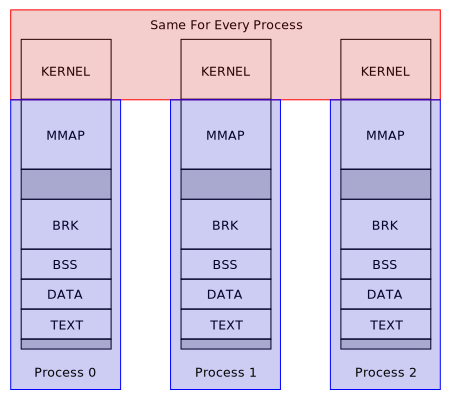
\includegraphics[width=0.45\linewidth]{memmap.png}
\end{center}
\begin{itemize}
  \item Ядро ОС отображается в адресное пространство каждого процесса:
  \begin{itemize}
    \item в таблице страниц каждого процесса есть записи для памяти ядра;
    \item эти записи должны запрещать непривилигерованный доступ к этой памяти.
  \end{itemize}
\end{itemize}
\end{frame}

\begin{frame}
\frametitle{Организация памяти процесса}
\begin{center}
  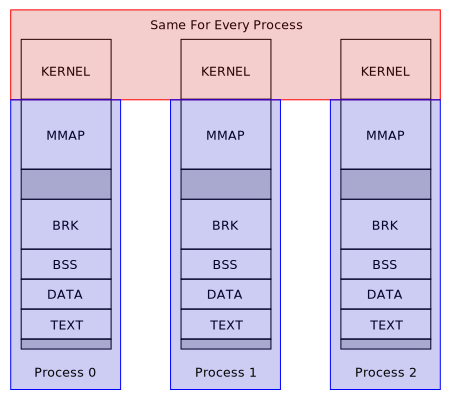
\includegraphics[width=0.45\linewidth]{memmap.png}
\end{center}
\begin{itemize}
  \item Остальная память у каждого процесса своя, но есть но:
  \begin{itemize}
    \item по обоюдному согласию процессы могут иметь общие участки памяти;
    \item память не обязательно физически разделена (хей-хей, page fault).
  \end{itemize}
\end{itemize}
\end{frame}

\begin{frame}
\frametitle{Финальные замечания про процессы}
\begin{itemize}
  \item Процесс - абстракция ОС созданная с использованием аппаратной поддержки:
  \begin{itemize}
    \item в объяснении выше использовалась таблица страниц для организации
    памяти;
    \item мы полагались на прерывания, для переключения потоков внутри процесса
    и между процессами.
  \end{itemize}
  \item Не трудно создать ОС, в которой такой абстракции не будет:
  \begin{itemize}
    \item например, если аппаратной поддержки нет или вам просто не нужна такая
    абстракция;
    \item примеры существуют: MS-DOS;
    \item абстракции не даются бесплатно - вы платите за это
    производительностью.
  \end{itemize}
\end{itemize}
\end{frame}

  \begin{frame}
\frametitle{Планирование потоков}
\begin{itemize}
  \item Мы знаем что-такое потоки и как между ними переключаться
  \begin{itemize}
    \item осталось разобраться когда и на какой конкретно поток переключаться.
  \end{itemize}
  \item Начнем с простой и нереалистичной задачи:
  \begin{itemize}
    \item мы заранее знаем все задачи, которые нужно выполнить;
    \item и про каждую задачу знаем сколько времени потребуется на выполнение;
    \item более того мы выполняем каждую задачу от начала до конца без
    переключений, т. е. нужно только определить порядок выполнения задач.
  \end{itemize}
\end{itemize}
\end{frame}

\begin{frame}
\frametitle{SJF 1/2}
\begin{columns}
  \begin{column}{0.5\linewidth}
    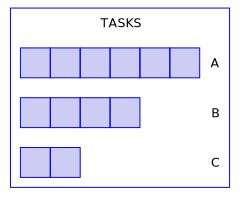
\includegraphics[width=0.9\linewidth]{sjf_tasks.png}
  \end{column}
  \begin{column}{0.5\linewidth}
    \includegraphics[width=0.9\linewidth]{sjf_schedule0.png}
    \begin{itemize}
      \item 3 задачи, по 6, 4 и 2 единиц;
      \item суммарно 12 единиц времени;
      \item среднее время ожидания заверешения:
      ${{6+10+12}\over{3}}=9.\left(3\right)$
    \end{itemize}
  \end{column}
\end{columns}
\end{frame}

\begin{frame}
\frametitle{SJF 2/2}
\begin{columns}
  \begin{column}{0.5\linewidth}
    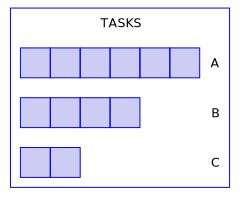
\includegraphics[width=0.9\linewidth]{sjf_tasks.png}
  \end{column}
  \begin{column}{0.5\linewidth}
    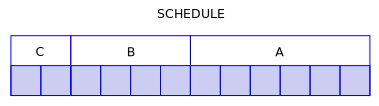
\includegraphics[width=0.9\linewidth]{sjf_schedule1.png}
    \begin{itemize}
      \item теже 3 задачи, по 6, 4 и 2 единиц;
      \item суммарно 12 единиц времени (о чудо!);
      \item среднее время ожидания заверешения:
      ${{2+6+12}\over{3}}=6.\left(6\right)$
    \end{itemize}
  \end{column}
\end{columns}
\end{frame}

\begin{frame}
\frametitle{Shortest Job First}
\begin{itemize}
  \item Упорядочив задачи по времени исполнения от меньшей к большей получим
  оптимальное по среднему времени ожидания расписание
  \begin{itemize}
    \item отсюда и Shortest Job First (SJF).
  \end{itemize}
\end{itemize}
\end{frame}

\begin{frame}
\frametitle{Блокировка потока}
\begin{itemize}
  \item Потоки могут быть заблокированы:
  \begin{itemize}
    \item поток может ожидать ввода от пользователя - даже самый быстрый
    пользователь очень медленный по сравнению с CPU;
    \item поток может ожидать получения данных по сети;
    \item поток может запросить доступ к медленному устройству и ждать
    прерывания от него (например, диск);
    \item другими словами поток может быть заблокирован в ожидании завершения
    операции ввода/вывода.
  \end{itemize}
  \item Заблокированным потокам нет смысла отдавать CPU:
  \begin{itemize}
    \item все что они могут делать, так это ждать завершения IO.
  \end{itemize}
\end{itemize}
\end{frame}

\begin{frame}
\frametitle{Динамическое создание и завершение}
\begin{itemize}
  \item Потоки создаются и завершаются динамически:
  \begin{itemize}
    \item новый поток может быть создан в любой момент;
    \item т. е. все потоки заранее не известны;
    \item существующий поток может завершиться в произвольный момент времени;
    \item т. е. мы не знаем время необходимое потоку для завершения.
  \end{itemize}
\end{itemize}
\end{frame}

\begin{frame}
\frametitle{Round Robin}
\begin{itemize}
  \item Самый простой вариант планирования в реалистичных условиях - отдавать
  процессор активным потокам по очереди:
  \begin{itemize}
    \item все задачи ожидающие CPU организованы в очередь;
    \item каждой задаче выделяется квант времени;
    \item задача снимается с CPU по истечении кванта;
    \item задача может отдать CPU самостоятельно перед истечением кванта;
    \item незаблокировавшаяся и незавершившаяся задача снятая с CPU возвращается
    в конец очереди.
  \end{itemize}
\end{itemize}
\end{frame}

\begin{frame}
\frametitle{Round Robin, pros}
\begin{itemize}
  \item Round Robin - является простым реалистичным алгоритмом планирования:
  \begin{itemize}
    \item выбор следующего потока требует $O\left(1\right)$;
    \item зная ограничение на количество потоков, мы можем ограничить
    максимальное время ожидания.
  \end{itemize}
  \item Гарантия, когда время реакции системы на событие (прерывание) жестко
  ограничено сверху - гарантия жесткого реального времени:
  \begin{itemize}
    \item т. е. Real Time на самом деле - это не про скорость;
    \item Round Robin сам по себе не нарушает гарантию реального времени.
  \end{itemize}
\end{itemize}
\end{frame}

\begin{frame}
\frametitle{Round Robin, cons 1/3}
\begin{itemize}
  \item IO Bounded поток - поток, работа которого ограничена скоростью IO:
  \begin{itemize}
    \item такие потоки часто не вырабатывают свой квант полностью, а отдают
    CPU раньше заблокировавшись на IO;
    \item типичный пример: текстовый редактор.
  \end{itemize}
  \item CPU Bounded поток - работа потока ограничивается скоростью CPU:
  \begin{itemize}
    \item такие потоки редко не вырабатывают свой квант полностью, они всегда
    хотят получить CPU в свое пользование;
    \item типичные примеры: численные расчеты, задачи рендеринга.
  \end{itemize}
\end{itemize}
\end{frame}

\begin{frame}
\frametitle{Round Robin, cons 2/3}
\begin{center}
  \includegraphics[width=0.8\linewidth]{rr0.png}
\end{center}
\begin{center}
  \includegraphics[width=0.8\linewidth]{rr1.png}
\end{center}
\end{frame}

\begin{frame}
\frametitle{Round Robin, cons 2/3}
\begin{center}
  \includegraphics[width=0.8\linewidth]{rr2.png}
\end{center}
\begin{center}
  \includegraphics[width=0.8\linewidth]{rr3.png}
\end{center}
\end{frame}

\begin{frame}
\frametitle{Round Robin, cons 3/3}
\begin{center}
  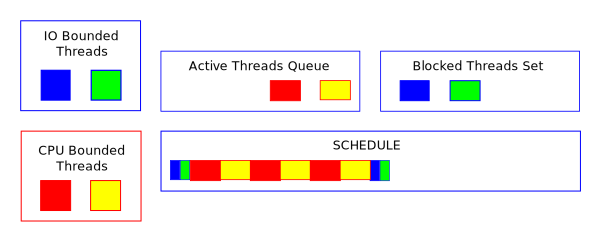
\includegraphics[width=0.8\linewidth]{rr4.png}
\end{center}
\begin{center}
  \includegraphics[width=0.8\linewidth]{rr5.png}
\end{center}
\end{frame}

\begin{frame}
\frametitle{Честность Round Robin}
\begin{itemize}
  \item IO Bounded задачи при Round Robin получают меньше CPU:
  \begin{itemize}
    \item они не вырабатывают свой квант и блокируются - не выработанное время
    никак не компенсируется.
  \end{itemize}
  \item IO Bounded задачи часто являются интерактивными, т. е. работают с
  пользователем, а пользователь не любит ждать
  \begin{itemize}
    \item однако когда поток разблокируется он встает в конец очереди и ждет
    пока вся очередь отработает.
  \end{itemize}
  \item Итого IO Bounded задачи получают меньше CPU, а задержка по доступу к CPU
  у них такая же как и у всех
  \begin{itemize}
    \item не все задачи одинаковые, и может потребоваться разделение задач на
    классы и приоритизация.
  \end{itemize}
\end{itemize}
\end{frame}

\begin{frame}
\frametitle{Completely Fair Scheduler 1/2}
\begin{itemize}
  \item Планировщик по-умолчанию в Linux Kernel
  \begin{itemize}
    \item пытается гарантировать идеальную честность отслеживая "виртуальное"
    отработанное время каждого потока;
    \item поток с нименьшим "виртуальным" временем получает CPU;
    \item выбор следующего потока требует $O\left(log n\right)$.
  \end{itemize}
\end{itemize}
\end{frame}

\begin{frame}
\frametitle{Completely Fair Scheduler 2/2}
\begin{itemize}
  \item Как обрабатывать разблокированные и новые потоки?
  \begin{itemize}
    \item нельзя просто верунть разблокированные задачи в очередь, т. к. их
    "виртуальное" время может сильно отстать от других и они станут "слишком
    приоритетными";
    \item для очереди потоков поддерживается "минимальное виртуальное" время,
    для новых и разблокированных задач проверяется, что их "виртуальное" время
    не сильно отстает от "минимального виртуального" времени.
  \end{itemize}
\end{itemize}
\end{frame}

\begin{frame}
\frametitle{Лотерейное планирование 1/2}
\begin{itemize}
  \item Самый "простой" способ обеспечить честность - рандомизация:
  \begin{itemize}
    \item выдадим каждому потоку набор лотерейных билетов;
    \item вероятность получения CPU в каждом "розыгыше" определяется количеством
    билетов у потока.
  \end{itemize}
  \item Статические и динамические приоритеты:
  \begin{itemize}
    \item потокам можно выдавать разное количество билетов согласно приоритету;
    \item кроме того, потоки могут временно передавать билеты друг другу и
    изменять свои приоритеты;
    \item например, поток \emph{A} пытается получить доступ к ресурсу \emph{X},
    но ресурс \emph{X} уже занят потоком \emph{B} - пусть \emph{A} передаст свои
    билеты \emph{B}, чтобы он раньше закончил работу с \emph{X}.
  \end{itemize}
\end{itemize}
\end{frame}

\begin{frame}
\frametitle{Лотерейное планирование 2/2}
\begin{itemize}
  \item При честной рандомизации возможны выбросы
  \begin{itemize}
    \item рандомизация гарантирует математическое ожидание времени CPU, но
    возможны отклонения от математического ожидания;
    \item чтобы ограничить отклонения, мы можем "удалять" выигравший билет;
    \item когда все билеты были "удалены", мы раздаем билеты заново;
    \item выбросы все еще возможны, но они ограничены (почти).
  \end{itemize}
\end{itemize}
\end{frame}


  \begin{frame}
  \begin{center}
  \Huge Q\&A
  \end{center}
  \end{frame}
\end{document}
